% !TEX TS-program = pdflatex
% !TEX encoding = UTF-8 Unicode

% This is a simple template for a LaTeX document using the "article" class.
% See "book", "report", "letter" for other types of document.

\documentclass[11pt]{article} % use larger type; default would be 10pt

\usepackage[utf8]{inputenc} % set input encoding (not needed with XeLaTeX)

%%% Examples of Article customizations
% These packages are optional, depending whether you want the features they provide.
% See the LaTeX Companion or other references for full information.

%%% PAGE DIMENSIONS
\usepackage{geometry} % to change the page dimensions
\geometry{a4paper} % or letterpaper (US) or a5paper or....
% \geometry{margin=2in} % for example, change the margins to 2 inches all round
% \geometry{landscape} % set up the page for landscape
%   read geometry.pdf for detailed page layout information

\usepackage{graphicx} % support the \includegraphics command and options

% \usepackage[parfill]{parskip} % Activate to begin paragraphs with an empty line rather than an indent

%%% PACKAGES
\usepackage{booktabs} % for much better looking tables
\usepackage{array} % for better arrays (eg matrices) in maths
\usepackage{paralist} % very flexible & customisable lists (eg. enumerate/itemize, etc.)
\usepackage{verbatim} % adds environment for commenting out blocks of text & for better verbatim
\usepackage{subfig} % make it possible to include more than one captioned figure/table in a single float
% These packages are all incorporated in the memoir class to one degree or another...

%%% HEADERS & FOOTERS
\usepackage{fancyhdr} % This should be set AFTER setting up the page geometry
\pagestyle{fancy} % options: empty , plain , fancy
\renewcommand{\headrulewidth}{0pt} % customise the layout...
\lhead{}\chead{}\rhead{}
\lfoot{}\cfoot{\thepage}\rfoot{}

%%% SECTION TITLE APPEARANCE
\usepackage{sectsty}


\allsectionsfont{\sffamily\mdseries\upshape} % (See the fntguide.pdf for font help)
% (This matches ConTeXt defaults)

%%% ToC (table of contents) APPEARANCE
\usepackage[nottoc,notlof,notlot]{tocbibind} % Put the bibliography in the ToC
\usepackage[titles,subfigure]{tocloft} % Alter the style of the Table of Contents
\renewcommand{\cftsecfont}{\rmfamily\mdseries\upshape}
\renewcommand{\cftsecpagefont}{\rmfamily\mdseries\upshape} % No bold!

%%% END Article customizations


\usepackage[bulgarian]{babel}
\usepackage{physics}
\usepackage{amsmath}
\usepackage{centernot}
\usepackage{url}
\usepackage{graphicx}
\graphicspath{ {.} }
\usepackage{amsfonts}
\usepackage{xcolor}

%%% The "real" document content comes below...

\title{Контекстно свободни граматики. Стекови автомати}
\author{Play4u}
%\date{} % Activate to display a given date or no date (if empty),
         % otherwise the current date is printed
         

\newcommand{\lrangle}[1]{\left\langle #1 \right\rangle}

\newcommand{\belongsTo}{\in}
\newcommand{\notBelongsTo}{\centernot\in}

\newcommand{\oversetModels}[1]{\overset{#1}{\models}}

\newcommand{\kda}{A = <Q, X, q_{0}, \delta, F>}
\newcommand{\cfg}{\Gamma = <\mathcal{N}, \mathcal{T}, \mathcal{S}, \mathcal{P}>}
\newcommand{\cfgVers}{G = \langle V, \Sigma, R, S \rangle}
\newcommand{\nsa}{A = <Q, X, Z, q_{0}, z_{0}, \delta, F>}

\newcommand{\italicBold}[1]{\textbf{\emph{#1}}}
\newcommand{\definition}{\italicBold{Дефиниция: }}
\newcommand{\theorem}{\italicBold{Теорема: }}
\newcommand{\lemma}{\italicBold{Лема: }}
\newcommand{\proof}{\italicBold{Доказателство: }}
\newcommand{\redText}[1]{\textcolor{red}{#1}}

\newcommand{\curlies}[1]{\{#1\}}
\newcommand{\overbar}[1]{\mkern 1.5mu\overline{\mkern-1.5mu#1\mkern-1.5mu}\mkern 1.5mu}

\newcommand{\enumNum}{\renewcommand{\theenumi}{\arabic{enumi}}}
\newcommand{\enumlet}{\renewcommand{\theenumi}{\alph{enumi}}} 

\begin{document}
\maketitle

\section{Булеви функции}
\definition Функция $\mathcal{F}_{2} = \curlies{f:J^{n}_{2} \to J^{n}_{2} | n = 1, 2, ...}$ наричаме \textit{булеви или двоични} Булевите функции на $n$ променливи означаваме с $\mathcal{F}^{n}_{2}$. \par

При стандартно подредени вектори от $\mathcal{F}^{n}_{2}$, всяка булева функция на $n$ променливи се задава еднозначно с вектор-стълва си с $2^{n}$ елемента. Очевидно $|\mathcal{F}^{n}_{2}| = 2^{2^n}$. При $n = 1$ и $n = 2$ имаме съответно 4 и 16 функции, които можем да изобразим така: 

\begin{table}[!ht]
\centering
\begin{tabular}{|l|llll|}
\hline
$x$ & $f_{0}$ & $f_{1}$ & $f_{2}$ &  $f_{3}$\\ \hline
0 & 0 & 0 & 1 & 1  \\
1 & 0 & 1 & 0 & 1 \\ \hline
\end{tabular}
\end{table}

При $n = 1$ имената на фунцкиите са следните: \\
\begin{itemize}
	\item $f_{0}(x)$ - константна 0. Означаваме я с $\tilde{0}$ за разлика от $0 \in J_{2}$; \\
	\item $f_{3}(x)$ - константна 1. Означаваме я с $\tilde{1}$ за разлика от $1 \in J_{2}$; \\
	\item $f_{1}(x)$ = $x$ - идентитетът \\
	\item $f_{2}(x)$ = $\bar{x}$ - отрицание на $x$; 
\end{itemize} \par

При $n = 2$ имаме: 
\begin{table}[!ht]
\centering
\begin{tabular}{|l|llll|}
\hline
$x$ & $f_{0}$ & $f_{1}$ & $f_{2}$ &  $f_{3}$\\ \hline
0 & 0 & 0 & 1 & 1  \\
1 & 0 & 1 & 0 & 1 \\ \hline
\end{tabular}
\end{table}

\newpage
При $n = 2$ функциите са следните:
\begin{center}
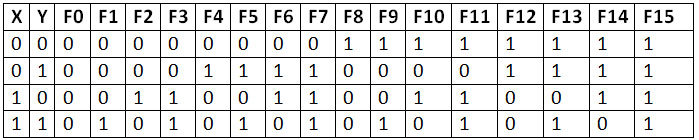
\includegraphics[scale=0.65]{twoVars.jpg}
\end{center}

Очевидно, всяка функция на $n$ променливи ще се появява и като функция на $n' > n$ променливи(т.е. $n' - n$ променливи ще са фиктивини или несъществени), при това много кратно - толкова пъти, по колкото начина можем да изберем фиктивните променливи. \par

Останалите функции от $\mathcal{F}^{2}_{2}$ зависят съществено и от двете си променливи. Ще ги означим и ще ги наричаме по следния начин:

\begin{itemize}
	\item $f_{1}(x,y) = x \wedge y = xy$ - \textit{конюкция}. Тази функция е частен случай при $q = 2$ на функциите $min(x_{1}, x_{2})$ и $x_{1}.x_{2}(mod\;q)$;\\  
	\item $f_{7}(x,y) = x \vee y $ - \textit{дизюнкция}. Тази функция е частен случай при $q = 2$ на функцията $max(x_{1}, x_{2})$;\\  
	\item $f_{6}(x,y) = x \oplus y$ - \textit{събиране на модул 2}. Тази функция е частен случай при $q = 2$ на функцията $x_{1} + x_{2}(mod\;q)$;\\
	\item $f_{9}(x,y) = x \equiv y$ - \textit{еквивалентност};\\  
	\item $f_{13}(x,y) = x \to y$ - \textit{импликация - $x$ следва от $y$};\\
	\item $f_{11}(x,y) = y \to x$ - \textit{обратна импликация - $y$ следва от $x$};\\ 
	\item $f_{14}(x,y) = y | x$ - \textit{функция(черта) на Шефер};\\
	\item $f_{8}(x,y) = y \downarrow x$ - \textit{функция(стрелка) на Пирс};\\       
\end{itemize}

\subsection{Свойства}
В сила са следните:
\enumlet
\begin{enumerate}
	\item \textit{комутативни свойства:}\\ 
		\centerline{$xy = yx, x \vee y = y \vee x, x \oplus y = y \oplus x$;} \\
	\item \textit{асоциативни свойства:}\\ 
		\centerline{$(xy)z = x(yz), (x \vee y) \vee z = x \vee (y \vee z), (x \oplus y)\oplus z = x \oplus (y \oplus z)$;} \\
	\item \textit{дистрибутивни свойства:}\\ 
		\centerline{$x(y \vee z) = xy \vee xz, x \vee yz = (x \vee y)(x \vee z), x(x \oplus z) = xy \oplus xz$;} \\
	\item \textit{идемпотентни свойства:}\\ 
		\centerline{$xx = x, x \vee x = x(x \oplus x) = \tilde{0}$;} \\
	\item \textit{свойства на отрицанието:}\\ 
		\centerline{$x\bar{x} = \tilde{0}, x \vee \bar{x} = \tilde{1}, x \oplus \bar{x} = \tilde{1}, \bar{\bar{x}} = x$;} \\
	\item \textit{свойства на константите:}\\ 
		\centerline{$x\tilde{0} = \tilde{0}, x\tilde{1} = x, x \vee \tilde{0} = x, x \vee \tilde{1} = \tilde{1}, x \oplus \tilde{0} = x, x \oplus \tilde{1} = \bar{x}$;} \\
	\item \textit{закони на Де Морган:}\\ 
		\centerline{$\overbar{x \vee y} = \bar{x} \wedge \bar{y},\overbar{x \wedge y} = \bar{x} \vee \bar{y}$;} \\
\end{enumerate}

\section{Формула над множество булеви функции \cite{fmiLectures}}

Дадено е изброимо множество от булеви променливи $\mathcal{X}$. Дадено е изброимо множество
от булеви фукции $\mathcal{F}$, чиито променливи са от $\mathcal{X}$. Дадена е крайна азбука $Z$, чиито символи
имат смисъл на цифри за някаква бройна система. Дадена е функция $\iota : \mathbb{N} \ to Z^{+}$, която е
биекция. Смисълът на $\iota$ е, бройната система. Нека\\
\centerline{$\redText{Y} = \curlies{\redText{f}, \redText{x}, \redText{(}, \redText{)}, \redText{,}}$}\\

В червено са символите от \redText{Y}, а в черно, метасимволите. Нека \\
\centerline{$\redText{\Sigma} = \redText{Y} \cup \redText{Z}$}\\

Формулите на $\mathcal{F}$ са точно тези низове от $\redText{\Sigma^{+}}$, които може да бъдат генерирани посредством краен брой прилагания на следните правила:

\enumNum
\begin{enumerate}
	\item Всеки низ $\redText{x \alpha}$ е формула, където $\redText{\alpha} \in \redText{\Sigma^{+}}$. Семантиката е $x_{j}$, където $x_{j} \in \mathcal{X}$ и $\iota(j) = \alpha$. \\
	\item За всяка функция $f_{k} \in \mathcal{F}$ нека $n$ е броят на нейните променливи, нека $\iota(k) = \redText{\alpha}$< нека $x_{1}, ..., x_{n}$ са нейните променливи и функцията е $f_{k}(x_{1}, ..., x_{n})$ и нека $\iota(j) = \redText{\beta_{j}}$ за $1 \leq j \leq n$, така че низът от $\redText{\Sigma^{+}}$, съотвестващ на $x_{j}$, да бъде $\redText{x\beta_{j}}$. Тогава низът \\
		\centerline{$\redText{f\alpha(x\beta_{1}, x\beta_{2}, ..., x\beta_{n})}$} \\
	е форума над $\mathcal{F}$ и нейната семантика, тоест нейната съотвестваща функция от $\mathcal{F}$ е $f_{k}(x_{1}, ..., x_{n})$.\\
	\item За $f_{k} \in \mathcal{F}$, нека $n$ е броят на нейните променливи, нека $\iota(k) = \redText{\alpha}$, нека $x_{1}, ..., x_{n}$ са нейните променливи и функцията е $f_{k}(x_{1}, ..., x_{n})$, и нека $\redText{\Phi_{1}, ..., \Phi_{n}}$ са формули над $\mathcal{F}$. Тогава \\
		\centerline{$\redText{f\alpha(\Phi_{1},\Phi_{2},..., \Phi_{n})}$}\\
	е формула над $\mathcal{N}$. Нейната семантика е функцията \\
	\centerline{$f_{k}(g_{1}, ..., g_{n})$} \\
	където $g_{j}$ е функцията от $\mathcal{F}$, съотвестваща на $\redText{\Phi_{j}}$, за $1 \leq j \leq n$.
	\item Няма други формули над $\mathcal{F}$.
\end{enumerate}

\begin{thebibliography}{1}
\bibitem{fmiLectures} 
Лекциите на ФМИ: \path{https://learn.fmi.uni-sofia.bg/pluginfile.php/50581/mod_resource/content/3/ff.pdf}
\end{thebibliography}

\section{Пълни множества}
\definition Множеството $F \subseteq \mathcal{F}_{q}$\textit{пълно}, ако $|F| = \mathcal{F}_{q}$.\\

Да се спрем първо на пълнотата на множества от булеви функции. \\

\definition Функцията $f(x, \sigma) = x ^{\sigma}$ дефинираме така \\
\centerline{$x^{\sigma} = 
	\begin{cases}
		x & \text{ ако } \sigma = 1 \\
		\bar{x} & \text{ ако } \sigma = 0 \\
	\end{cases}
$}\\
\lemma $x^{\sigma} = 1 \leftrightarrow x^{\sigma} = \sigma$

\section{Разлагане на булева функция по част от променливите}
\theorem Нека са избрани $i, 1 \leq i \leq n$ от променливите на функцията $f(x_{1}, x_{2}, ..., x_{n}) \in \mathcal{F}_{2}$ Без ограничение на общността, нека това са първите $i$ променливи. Тогава \\

\centerline{$f(x_{1}, x_{2}, ..., x_{n}) = \underset{\forall \sigma_{1}\sigma_{2}...\sigma_{i}}{\bigvee} x_{1}^{\sigma_1}x_{2}^{\sigma_2} ... x_{i}^{\sigma_i} f(\sigma_{1}, \sigma_{2}, ..., \sigma_{i}, x_{i+1}, ..., x_{n})$}

\proof Да означим с $g(x_{1}, x_{2}, ..., x_{n})$ функцията, определена от дясната част на равенството. Да пресметнем стойностите на функциите $f$ и $g$ за произволен вектор $a_{1}, a_{2}, ..., a_{n} \in J^{n}_{2}$. Вляво получаваме $f(a_{1}, a_{2}, ..., a_{n})$. От лемата, която описахме по-горе, следва че от всички $2^{i_\iota}$ елементарни конюкции $x_{1}^{\sigma_1} x_{2}^{\sigma_2} ... x_{i}^{\sigma_i}$, участващи в дясната част, само една има стойност 1 - тази, при която $\sigma_{j} = a_{j}, j = 1, 2, ..., i$. Останалите елементарни конюкции имат стойност 0 и анулират съответните членове на многократната дизюнкция. Така за стойността на дясната част получаваме: \\

\centerline{$g(a_{1}, a_{2}, ..., a_{n}) = $}
\centerline{$ = a_{1}^{a_1} a_{2}^{a_2} ... a_{i}^{a_i} f(a_{1}, a_{1}, ..., a_{i}, a_{i+1}, ..., a_{n})\vee \tilde{0} = $}
\centerline{$ = \tilde{1}f(a_{1}, a_{2}, ..., a_{i}, a_{i+1},..., a_{n}) = f(a_{1}, a_{2}, ..., a_{n})$}.

Следователно, функциите от двете страни на равенството съвпадат.

\section{Теорема на Бул}
\theorem Множеството $\curlies{x \vee y, xy, \bar{x}}$ е пълно\\

\proof (Опционално?)Ще покажем, че $\forall \in \mathcal{F}_{2}$ е в сила $f \in [\curlies{x \vee y, xy, \bar{x}}]$, т.е. можем да представим $f$ с формула над $\curlies{x \vee y, xy, \bar{x}}$.

\enumNum
\begin{enumerate}
	\item Нека $f = \tilde{0}$. Тогава $f(x) = x\bar{x}$ и следователно $f$ се представя с форумла над $\curlies{x \vee y, xy, \bar{x}}$. \\
	\item Нека $f \neq \tilde{0}$. Разлагаме $f(x_{1}, x_{2}, ..., x_{n})$ по всичките $n$ променливи и получаваме \\
		\centerline{$f(x_{1}, x_{2}, ..., x_{n}) = \underset{\forall \sigma_{1}\sigma_{2}...\sigma_{n}}{\bigvee}x_{1}^{\sigma_1} x_{2}^{\sigma_2} ... x_{n}^{\sigma_n} f(\sigma_{1}, \sigma_{2}, ..., \sigma_{n})$.}
\end{enumerate}

Ако $f(\sigma_{1}, \sigma_{2}, ..., \sigma_{n}) = 0$, съответният член в дясната част се анулира и съгласно свойствата, доказани по-горе, може да не участва във формулата. Ако пък $f(\sigma_{1}, \sigma_{2}, ..., \sigma_{n}) = 1$, то $x_{1}^{\sigma_1}x_{2}^{\sigma_2}... x_{n}^{\sigma_n} f(\sigma_{1}, \sigma_{2}, ..., \sigma_{n}) = x_{1}^{\sigma_1}x_{2}^{\sigma_2}... x_{n}^{\sigma_n}$. Така получаваме \\ 

\centerline{$f(x_{1}, x_{2}, ..., x_{n}) =   \bigvee_{\substack{\forall \sigma_{1} \sigma{2}...\sigma{n} \\ f(\sigma_{1} \sigma{2}...\sigma{n}) = 1}} x_{1}^{\sigma_1}x_{2}^{\sigma_2}...x_{n}^{\sigma_n}$}

което е формула над $\curlies{x \vee y, xy, \bar{x}}$.

\section{Теорема на Пост-Яблонски}
\theorem Нека $F \subseteq \mathcal{F}^{n}_{2}$. Множеството $F$ е пълно $\leftrightarrow$, когато \\
\centerline{$F\not\subseteq T_{0}\;\&\;F \not\subseteq T_{1}\;\&\;F \not\subseteq S\;\&\;F \not\subseteq M\;\&\;F \not\subseteq L$}\\
\centerline{\textit{Insert proof here}}

\end{document} 